%%%%%%%%%%%%%%%%%%%%%%%%%%%%%%%%%%%%%%%%%%%%%%%%%%%%%%%%%%%%%%%%%%%%
% Authors: A. Herrera-Poyatos, F. Herrera
% Tittle: Algoritmo memético equilibrado con diversificación voraz
% 							 CAEPIA 2015
%%%%%%%%%%%%%%%%%%%%%%%%%%%%%%%%%%%%%%%%%%%%%%%%%%%%%%%%%%%%%%%%%%%%

\section{Big Data}

	\subsection*{¿Qué es Big Data?}

		\begin{frame}{Definición}
			\kern-0.5cm
			\begin{figure}
				\centering
				\textbf{Conjuntos de datos masivos}
				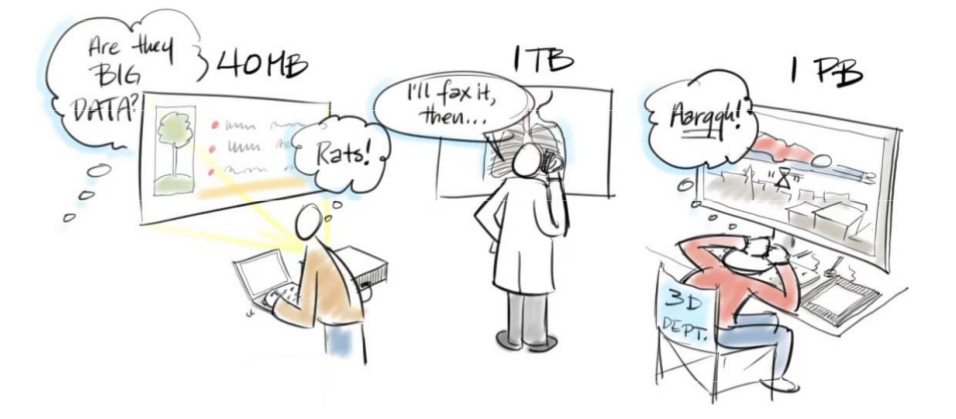
\includegraphics[width=0.85\textwidth]{./Images/what-is-big-data.png}
			\end{figure}

			\fontsize{8}{8}\selectfont	
			\begin{tcolorbox}[colback=ChetwodeBlue!10,colframe=ChetwodeBlue!60]
				``Un problema sobre datos entra en el ámbito de Big Data cuando la aplicación de las actuales tecnologı́as no permite al usuario obtener soluciones rápidas, efectivas en costo y de calidad. ''
				\begin{flushright}
					Michael J. Franklin, Universidad de Berkley 
				\end{flushright}
			\end{tcolorbox}
		\end{frame}
		
		\begin{frame}{Características: las 3 Vs de Big Data}
			\kern -0.5cm
			\fontsize{6}{8}\selectfont
			\begin{tikzpicture}
				\node (img1) {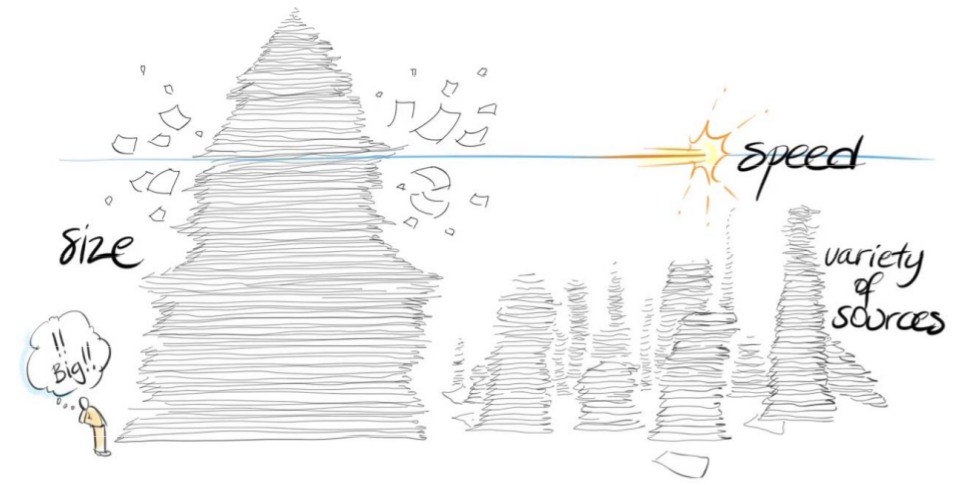
\includegraphics[width=\textwidth]{./Images/big-data-vs.png}};
				\node [above left = 2.2cm and 2.5cm of $(img1)$] (img2) {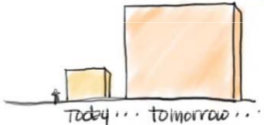
\includegraphics[width=0.3\textwidth]{./Images/escalabilidad.png}};
				\node [above = 8mm of $(img2)$] (es) {\textbf{Escalabilidad}};
				\node [fill=Grandis!80, circle,inner sep=0.5pt, text width=1.35cm, align=center, above right = 2cm and 1.8cm of $(img1)$] (vel) {Velocidad};
				\node [fill=TurkishRose!80, circle,inner sep=0.5pt, text width=1.35cm, align=center, right= 1.6cm of $(vel)$] (var) {Variedad};
				\node [fill=ChetwodeBlue!80, circle, inner sep=0.5pt, text width=1.35cm, align=center, above = 9mm of $(vel)!0.5!(var)$] (vol) {Volumen};
				\node [fill=Jaguar!85, circle, inner sep=0.5pt, text width=1.5cm, align=center, below = 4mm of $(vol)$] (bd) {\color{white}{\textbf{Big Data}}};
			\end{tikzpicture}

		\end{frame}

	
	\subsection*{Big Data e ingeniería de servidores}
	
		\begin{frame}{\large Cómo trabajar en Big Data: computación de altas prestaciones}
			
			
			\begin{columns}
				\column{0.65\textwidth}
				\fontsize{8.5}{8}\selectfont

				\begin{tcolorbox}[colback=ChetwodeBlue!10,colframe=ChetwodeBlue!60]
					Agregación de varios computadores con el fin de obtener una mayor potencia y rendimiento
				\end{tcolorbox}
				{\begin{center}\large\color{ChetwodeBlue}Programación distribuida\end{center}}
				\kern-5mm
				\begin{figure}
					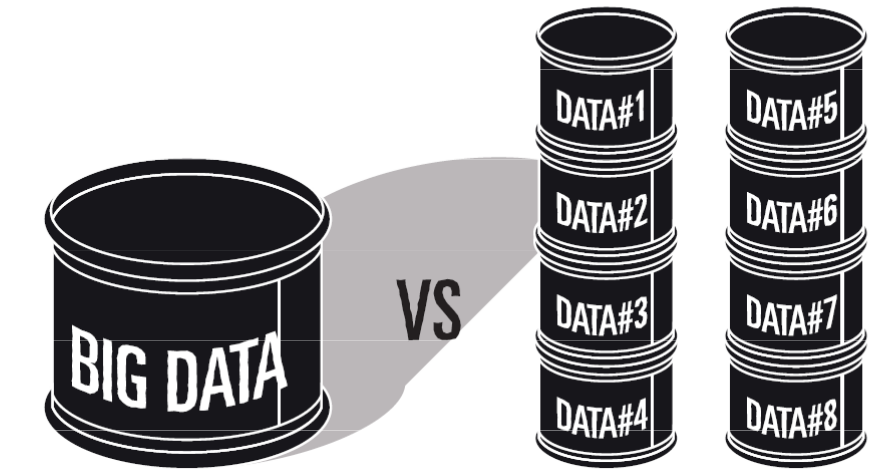
\includegraphics[width=\textwidth]{./Images/bloques.png}
				\end{figure}

				\column{0.35\textwidth}
				\begin{figure}
					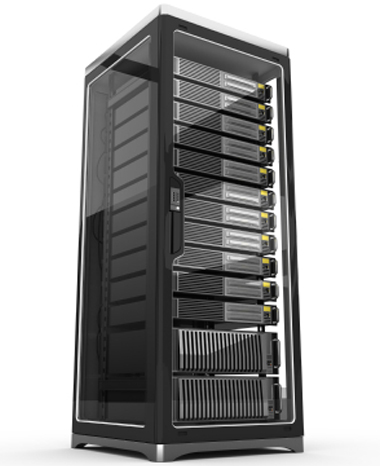
\includegraphics[width=\textwidth]{./Images/cluster.jpg}
				\end{figure}
				\fontsize{9}{8}\selectfont	
				\textbf{Selección de un servidor}

			\end{columns}
			
		\end{frame}